\begin{frame}[t,fragile]{関数値の評価}
  \begin{itemize}
    %\setlength{\itemsep}{1em}
  \item $\displaystyle f(x_1,x_2,x_3) = \frac{(x_1 - \exp(x_2)) x_3 \exp(x_2)}{x_3 \exp(x_2) + 1}$
  \item $(x_1,x_2,x_3)=(2,0,1)$における$f(x_1,x_2,x_3)$の値の評価
    \begin{itemize}
    \item $x_1 \leftarrow 2$
    \item $x_2 \leftarrow 0$
    \item $x_3 \leftarrow 1$
    \item $v_1 \leftarrow \exp(x_2) = 1$
    \item $v_2 \leftarrow x_1 - v_1 = 1$
    \item $v_3 \leftarrow v_1 \times x_3 = 1$
    \item $v_4 \leftarrow v_2 \times v_3 = 1$
    \item $v_5 \leftarrow v_3 + 1 = 2$
    \item $f \leftarrow v_4 / v_5 = 1/2$
    \end{itemize}
    \vspace*{-7em} \hfill \resizebox{.3\textwidth}{!}{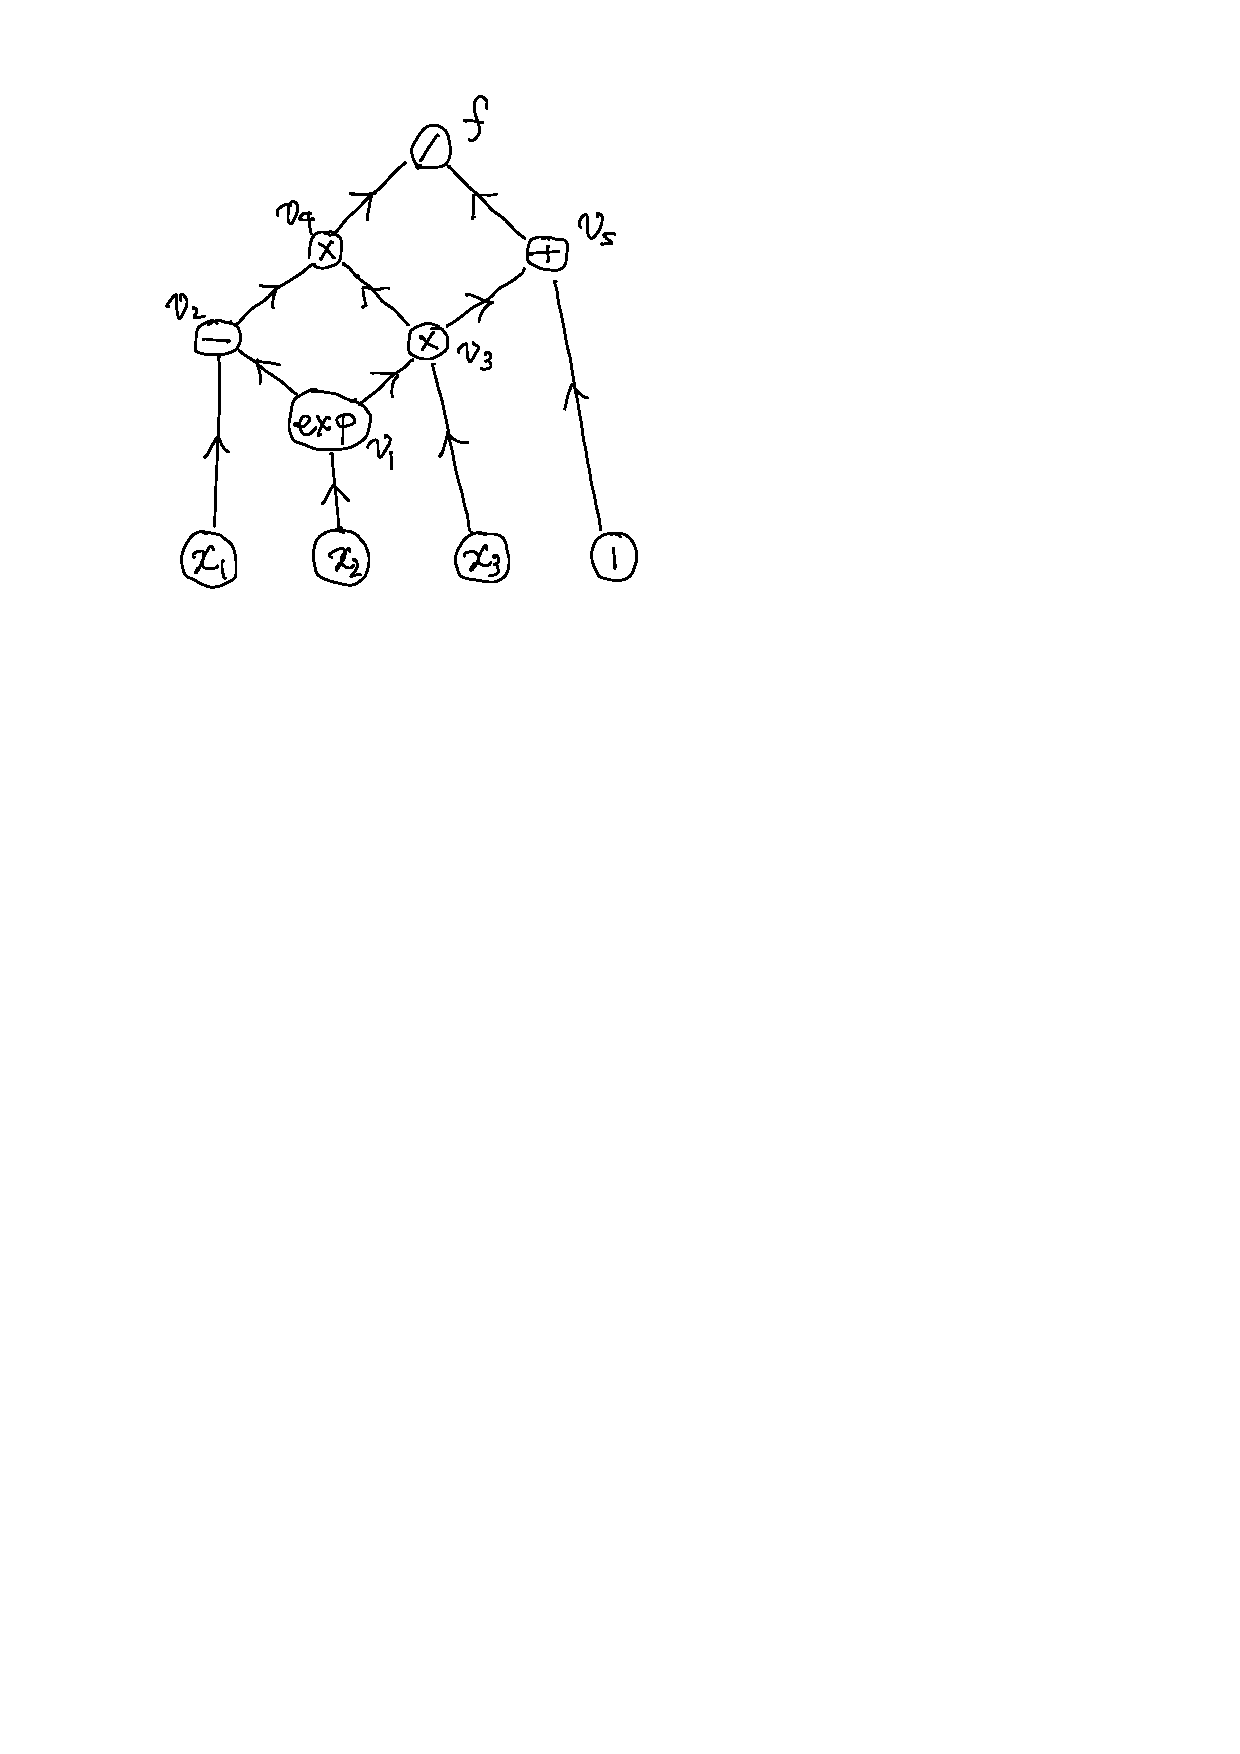
\includegraphics{image/compgraph.pdf}}
  \end{itemize}
\end{frame}
